\documentclass[11pt,class=report,crop=false]{standalone}
\usepackage[screen]{../python}
\begin{document}



%====================================================================
\chapitre{Dynamic images}
%====================================================================

\objectifs{We will distort images. By repeating these distortions, the images become blurred. But by a miracle after a certain number of repetitions the original image reappears!}

\index{image}

%%%%%%%%%%%%%%%%%%%%%%%%%%%%%%%%%%%%%%%%%%%%%%%%%%%%%%%%%%%%%%%%
%%%%%%%%%%%%%%%%%%%%%%%%%%%%%%%%%%%%%%%%%%%%%%%%%%%%%%%%%%%%%%%%

\begin{cours}[Transformation of the photo booth]

We start from an array $n\times n$, with $n$ even, each element of the table represents a pixel. The rows are indexed from $i=0$ to $i=n-1$, the columns from $j=0$ to $j=n-1$.
From this image we calculate a new image by moving each pixel according to a transformation, called the \defi{photo booth transformation}.

We cut the original image into small squares of size $2\times2$.
Each small square is therefore composed of four pixels. Each of these pixels is sent to four different locations in the new image:
the pixel at the top left remains in an area at the top left, the pixel at the top right of the small square, is sent to an area at the top right of the new image,...

\myfigure{0.7}{
\tikzinput{fig-images-1}
}

For example, the pixel in position $(1,1)$ (symbolized by the letter \mot{D}) is sent in position $(4,4)$.

\medskip

Let's explain this principle through formulas. For each couple $(i,j)$, we calculate its image $(i',j')$ by the photo booth transformation  according to the following formulas:
\begin{itemize}
  \item If $i$ and $j$ are even: $(i',j') = (i//2,j//2)$.
  \item If $i$ is even and $j$ is odd: $(i',j') = (i//2,(n+j)//2)$.  
  \item If $i$ is odd and $j$ is even: $(i',j') = ((n+i)//2,j//2)$.
  \item If $i$ and $j$ are odd: $(i',j') = ((n+i)//2,(n+j)//2)$.
\end{itemize}


\medskip

Here is an example of an array $4\times 4$ before (left) and after (right) the transformation of the photo booth. 
$$\begin{array}{cccc} 
  1& 2& 3& 4\\ 
  5& 6& 7& 8\\  
  9&10&11&12\\  
 13&14&15&16  
\end{array}\qquad\qquad  
\begin{array}{cccc} 
  1& 3& 2& 4\\  
  9&11&10&12\\  
  5& 7& 6& 8\\  
 13&15&14&16
\end{array}$$

Here is an image $256 \times 256$ and its first transformation:

\begin{center}
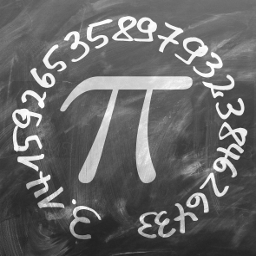
\includegraphics[scale=\myscale,scale=0.4]{images_chapter/pi_gimp_new_photo_0.png}\qquad\qquad
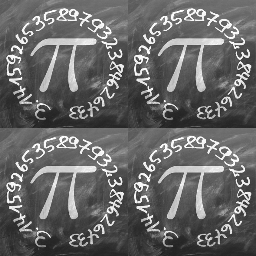
\includegraphics[scale=\myscale,scale=0.4]{images_chapter/pi_gimp_new_photo_1.png}
\end{center}

Here is what happens if you repeat the photo booth transformation several times:
\begin{center}
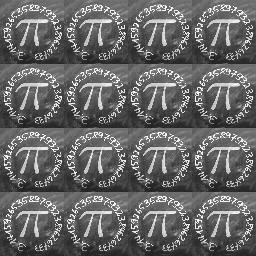
\includegraphics[scale=\myscale,scale=0.3]{images_chapter/pi_gimp_new_photo_2.png}\qquad
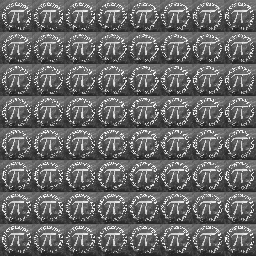
\includegraphics[scale=\myscale,scale=0.3]{images_chapter/pi_gimp_new_photo_3.png}\qquad
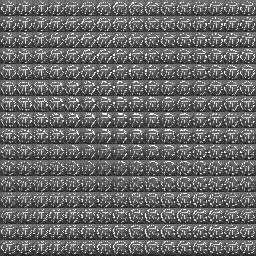
\includegraphics[scale=\myscale,scale=0.3]{images_chapter/pi_gimp_new_photo_4.png}
\end{center}
\begin{center}
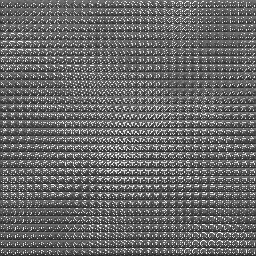
\includegraphics[scale=\myscale,scale=0.3]{images_chapter/pi_gimp_new_photo_5.png}\qquad
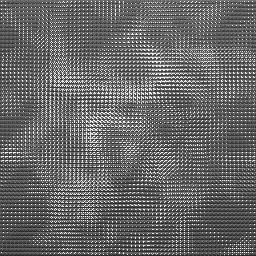
\includegraphics[scale=\myscale,scale=0.3]{images_chapter/pi_gimp_new_photo_6.png}\qquad
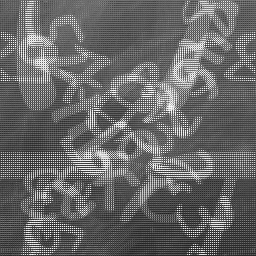
\includegraphics[scale=\myscale,scale=0.3]{images_chapter/pi_gimp_new_photo_7.png}\qquad
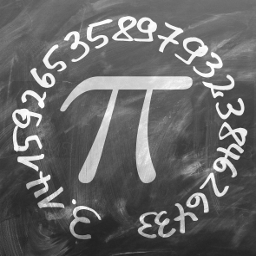
\includegraphics[scale=\myscale,scale=0.3]{images_chapter/pi_gimp_new_photo_8.png}
\end{center}
The image becomes more and more blurred, but after some number of repetitions of the transformation, we fall back on the original image!
\end{cours}




%%%%%%%%%%%%%%%%%%%%%%%%%%%%%%%%%%%%%%%%%%%%%%%%%%%%%%%%%%%%%%%%
% Activity 1 - Photomaton transformation
%%%%%%%%%%%%%%%%%%%%%%%%%%%%%%%%%%%%%%%%%%%%%%%%%%%%%%%%%%%%%%%%


\begin{activite}[Transformation of the photo booth]

\objectifs{Goal: program the transformation of the photo booth that decomposes an image into sub-pictures. When this transformation is iterated, the image gradually disintegrates, then suddenly re-formed.}



\begin{enumerate}
  \item Program a function \ci{transformation(i,j,n)} that realize the formula of the photo booth transformation and returns the coordinates $(i',j')$ of the pixel image $(i,j)$.
  
  For example, \ci{transformation(1,1,8)} returns \ci{(4,4)}.
  
  \item Program a function \ci{photo_booth(array)} that returns the table calculated after transformation.

For example, the array on the left is transformed into the array on the right.
$$\begin{array}{cccc} 
  1& 2& 3& 4\\ 
  5& 6& 7& 8\\  
  9&10&11&12\\  
 13&14&15&16  
\end{array}\qquad\qquad
\begin{array}{cccc} 
  1& 3& 2& 4\\  
  9&11&10&12\\  
  5& 7& 6& 8\\  
 13&15&14&16
\end{array}$$

  \emph{Hints.} You can initialize a new table with the command:  
  \mycenterline{\ci{new_array = [[0 for j in range(n)] for i in range(n)]}}
  
  Then fill it with commands of the type: 
  \mycenterline{\ci{new_array[ii][jj] = array[i][j]}}

  \item Program a function \ci{photo_booth_iterate(array,k)} that returns the table calculated after $k$ iterations of the photo booth transformation.
  
  \item \emph{To be finished after completing activity 2.}
  
  Program a function \ci{photo_booth_images(image_name,kmax)} that calculates the images corresponding to the transformation, for all iterations from $k=1$ to $k=k_{\max}$.
  
  \item Experiment for different values of the size $n$, to see after how many iterations we find the original image.
  
\end{enumerate}

Here is the starting image size $256 \times 256$ and the images obtained by iterations of the photo booth transformation for $k=1$ up to $k=8$. After $8$ iterations we find the initial image again.
\begin{center}
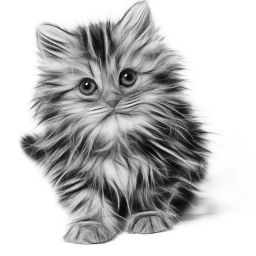
\includegraphics[scale=\myscale,scale=0.4]{images_chapter/cat_gimp_new_photo_0.png}
\end{center}
\begin{center}
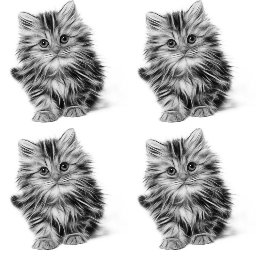
\includegraphics[scale=\myscale,scale=0.3]{images_chapter/cat_gimp_new_photo_1.png}\qquad
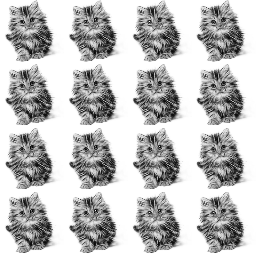
\includegraphics[scale=\myscale,scale=0.3]{images_chapter/cat_gimp_new_photo_2.png}\qquad
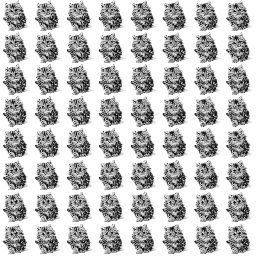
\includegraphics[scale=\myscale,scale=0.3]{images_chapter/cat_gimp_new_photo_3.png}\qquad
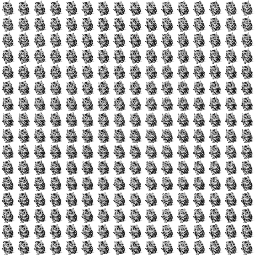
\includegraphics[scale=\myscale,scale=0.3]{images_chapter/cat_gimp_new_photo_4.png}
\end{center}
\begin{center}
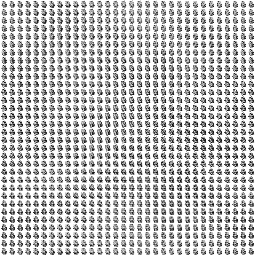
\includegraphics[scale=\myscale,scale=0.3]{images_chapter/cat_gimp_new_photo_5.png}\qquad
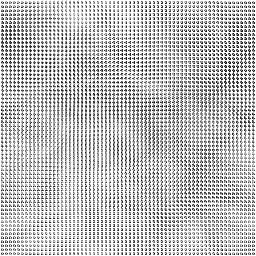
\includegraphics[scale=\myscale,scale=0.3]{images_chapter/cat_gimp_new_photo_6.png}\qquad
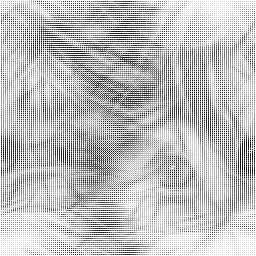
\includegraphics[scale=\myscale,scale=0.3]{images_chapter/cat_gimp_new_photo_7.png}\qquad
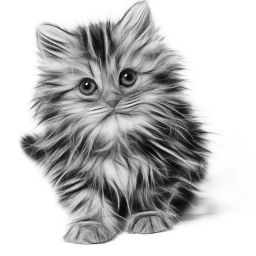
\includegraphics[scale=\myscale,scale=0.3]{images_chapter/cat_gimp_new_photo_8.png}
\end{center}


\end{activite}


%%%%%%%%%%%%%%%%%%%%%%%%%%%%%%%%%%%%%%%%%%%%%%%%%%%%%%%%%%%%%%%%
% Activity 2 - Conversion of table/image
%%%%%%%%%%%%%%%%%%%%%%%%%%%%%%%%%%%%%%%%%%%%%%%%%%%%%%%%%%%%%%%%


\begin{activite}[Conversion array/image]

\objectifs{Goal: switch from an array to an image file and vice versa. The format to display the images is the format \og{}pgm\fg{} which has been manipulated in the chapter \og{}Files\fg{}.}

\index{pbm@\emph{pbm/pgm/ppm}}

\begin{enumerate}
  \item \textbf{Array to image.}
  
  Program a function \ci{array_to_image(array,image_name)} that writes an image file in format \og{}pgm\fg{} from a grayscale table.
  
\begin{center}
\begin{minipage}{0.3\textwidth}
\begin{lstlisting}
P2
5 5
255
128 192 128 192 128
224   0 228   0 224
228 228 228 228 228 
224  64  64  64 224 
192 192 192 192 192 
\end{lstlisting}
\end{minipage}
\begin{minipage}{0.3\textwidth}
\begin{center}

\includegraphics[scale=\myscale,scale=0.15]{input/ecran-test-pgm}
\end{center}
\end{minipage}
\end{center}
For example with \ci{array = [ [128,192,128,192,128], [224,...] ]}, the command \ci{array_to_image(array,"test")} writes a file \ci{test.pgm} (on the left) that would be displayed as the image on the right.

  
  
  \item \textbf{Image to array.} 
  
  Program a function \ci{image_to_array(image_name)} 
  which from an image file in format \og{}pgm\fg{}, returns an array of gray levels.
\end{enumerate}

\end{activite}


%%%%%%%%%%%%%%%%%%%%%%%%%%%%%%%%%%%%%%%%%%%%%%%%%%%%%%%%%%%%%%%%
%%%%%%%%%%%%%%%%%%%%%%%%%%%%%%%%%%%%%%%%%%%%%%%%%%%%%%%%%%%%%%%%
\begin{cours}[Baker's transformation]

We start from an array $n\times n$, with $n$ even, each element representing a pixel. 
We will apply two elementary transformations each time:

\begin{itemize}
  \item \textbf{Stretching.} The principle is as follows: the first two lines (each with a length of $n$) produce a single line with a length of $2n$ by mixing the values of each line by alternating an upper element and a lower element.

\medskip
 
\myfigure{1}{
\tikzinput{fig-images-2}
}

Here is how two lines mix into one:
\myfigure{1}{
\tikzinput{fig-images-2bis}
}  

\medskip

\emph{Formulas.} An element at position $(i,j)$ of the target array, corresponds to an element $(2i,j//2)$ (if $j$ is even) or $(2i+1,j//2)$ (if $j$ is odd) of the source array, with here $0 \le i < \frac n2$ and $0 \le j < 2n$.

\medskip

\emph{Example.} Here is an array $4 \times 4$ on the left, and the stretched array $2 \times 8$ on the right.
The rows $0$ and $1$ on the left give the row $0$ on the right.
The rows $2$ and $3$ on the left give the row $1$ on the right.
$$\begin{array}{cccc} 
  1& 2& 3& 4\\ 
  5& 6& 7& 8\\  
  9&10&11&12\\  
 13&14&15&16  
\end{array}\qquad\qquad 
\begin{array}{cccccccc} 
  1& 5& 2& 6& 3& 7& 4& 8  \\
  9&13&10&14&11&15&12&16
\end{array}$$
  
  \item \textbf{Fold.} The principle is as follows: the right part of a stretched array is turned upside down, then added under the left part. Starting from an array $\frac n2 \times 2n$ you get an array $n \times n$.

 
\myfigure{0.7}{
\tikzinput{fig-images-3}
}  

\emph{Formulas.} 
For $0 \le i < \frac n2$ and $0 \le j < n$ the elements in position $(i,j)$ of the array are kept.
For $\frac n2 \le i < n$ and $0 \le j < n$ an element of the array 
$(i,j)$, corresponds to an element $\big(\frac{n}{2} - i - 1,2n-1-j\big)$ of the source array. 


\emph{Example.} 
From the stretched array $2 \times 8$ on the left, we obtain a folded array $4 \times 4$ on the right. 
$$ 
\begin{array}{cccccccc} 
  1& 5& 2& 6& 3& 7& 4& 8  \\
  9&13&10&14&11&15&12&16
\end{array}\qquad\qquad
\begin{array}{cccc} 
  1& 5& 2& 6\\ 
  9& 13& 10& 14\\  
  16&12&15&11\\  
  8&4&7&3  
\end{array}$$
\end{itemize}


The \defi{transformation of the baker} is the succession of a stretching and a folding. Starting from an array $n \times n$ we still get an array $n \times n$.


Let's see an example of the action of several transformations of the baker.
On the left the initial image size $128 \times 128$, then the result of $k=1,2,3$ iterations. 

\begin{center}

\includegraphics[scale=\myscale,scale=0.65]{images_chapter/surf_gimp_new_baker_0.png}\qquad
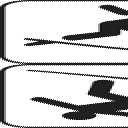
\includegraphics[scale=\myscale,scale=0.65]{images_chapter/surf_gimp_new_baker_1.png}\qquad
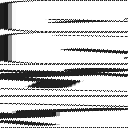
\includegraphics[scale=\myscale,scale=0.65]{images_chapter/surf_gimp_new_baker_2.png}\qquad
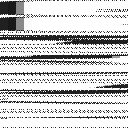
\includegraphics[scale=\myscale,scale=0.65]{images_chapter/surf_gimp_new_baker_3.png}
\end{center}


Here are the images for $k=12,13,14,15$ iterations:

\begin{center}
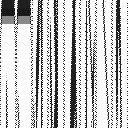
\includegraphics[scale=\myscale,scale=0.65]{images_chapter/surf_gimp_new_baker_12.png}\qquad
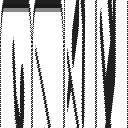
\includegraphics[scale=\myscale,scale=0.65]{images_chapter/surf_gimp_new_baker_13.png}\qquad
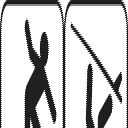
\includegraphics[scale=\myscale,scale=0.65]{images_chapter/surf_gimp_new_baker_14.png}\qquad

\includegraphics[scale=\myscale,scale=0.65]{images_chapter/surf_gimp_new_baker_15.png}
\end{center}

\end{cours}

%%%%%%%%%%%%%%%%%%%%%%%%%%%%%%%%%%%%%%%%%%%%%%%%%%%%%%%%%%%%%%%%
% Activity 3 - Baker processing
%%%%%%%%%%%%%%%%%%%%%%%%%%%%%%%%%%%%%%%%%%%%%%%%%%%%%%%%%%%%%%%%


\begin{activite}[Baker's transformation]

\objectifs{Goal: program a new transformation that stretches and folds an image. Once again, the image becomes more and more distorted but, after a certain number of iterations, we find the original image again.}


\begin{enumerate}
  \item Program a function \ci{baker_stretch(array)} that returns a new array obtained by \og{}stretching\fg{} the table given as input.



    \item Program a function \ci{baker_fold(array)} that returns a table obtained by \og{}folding\fg{} the table given as input.
  
  
   \item Program a function \ci{baker_iterate(array,k)} that returns the table calculated after $k$ iterations of the baker's transformation.
  
  For example, here is a table $4 \times 4$ on the left, its image by the transformation ($k=1$) and its image after a second transformation ($k=2$).
  
 $$\begin{array}{cccc} 
  1& 2& 3& 4\\ 
  5& 6& 7& 8\\  
  9&10&11&12\\  
 13&14&15&16  
\end{array}\qquad\qquad  
 \begin{array}{cccc} 
  1& 5& 2& 6\\ 
  9& 13& 10& 14\\  
  16&12&15&11\\  
  8&4&7&3  
\end{array}\qquad\qquad  
 \begin{array}{cccc} 
   1&    9&    5&   13 \\ 
 16&    8&   12&    4\\  
  3&   11&    7&   15\\  
 14&    6&   10&    2
\end{array}
$$ 
  \item Program a function  \ci{baker_images(image_name,kmax)} that calculates the images corresponding to the transformation of the baker, with iterations ranging from $k=1$ to $k=k_{\max}$.
  
  \item Experiment for different values of the size $n$, to see after how many iterations we find the original image. 
  
  \emph{Caution!} It sometimes takes a lot of iterations to get back to the original image. For example with $n=4$, we find the starting image after $k=5$ iterations; with $n=256$ it is $k=17$. Conjecture a return value in the case where $n$ is a power of $2$. However, for $n=10$, you need $k = 56\,920$ iterations!
   
  
\end{enumerate}

Here is an example with an image of size $256 \times 256$, first the initial image, then one transformation ($k=1$) and a second iteration ($k=2$).
\begin{center}
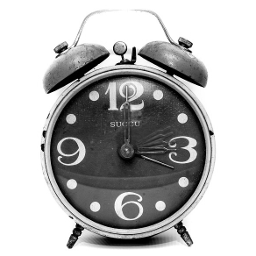
\includegraphics[scale=\myscale,scale=0.4]{images_chapter/clock_gimp_new_baker_0.png}\qquad
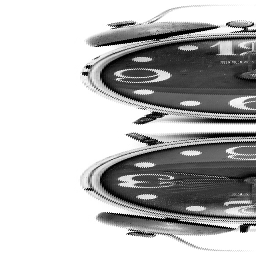
\includegraphics[scale=\myscale,scale=0.4]{images_chapter/clock_gimp_new_baker_1.png}\qquad
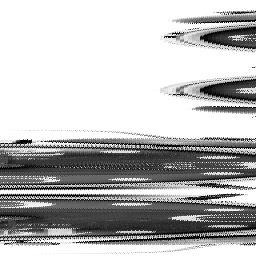
\includegraphics[scale=\myscale,scale=0.4]{images_chapter/clock_gimp_new_baker_2.png}
\end{center}
$k=3,4,5$ :
\begin{center}
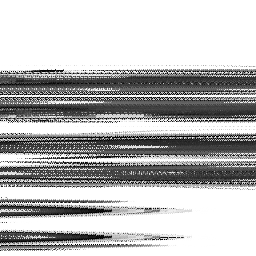
\includegraphics[scale=\myscale,scale=0.4]{images_chapter/clock_gimp_new_baker_3.png}\qquad
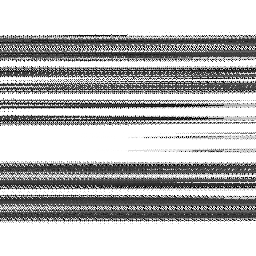
\includegraphics[scale=\myscale,scale=0.4]{images_chapter/clock_gimp_new_baker_4.png}\qquad
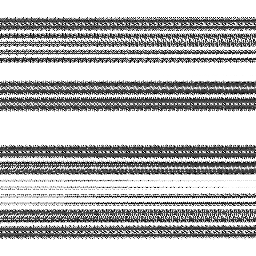
\includegraphics[scale=\myscale,scale=0.4]{images_chapter/clock_gimp_new_baker_5.png}
\end{center}

$k=15,16,17$ :
\begin{center}
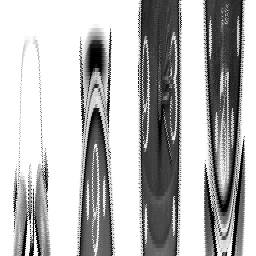
\includegraphics[scale=\myscale,scale=0.4]{images_chapter/clock_gimp_new_baker_15.png}\qquad
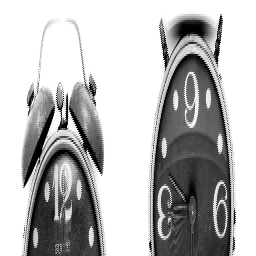
\includegraphics[scale=\myscale,scale=0.4]{images_chapter/clock_gimp_new_baker_16.png}\qquad
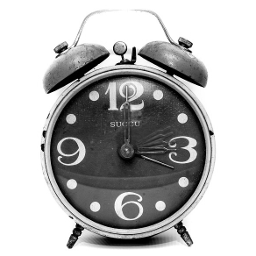
\includegraphics[scale=\myscale,scale=0.4]{images_chapter/clock_gimp_new_baker_17.png}
\end{center}

For $k=17$ you find the original image!

\end{activite}


This chapter is based on the article \og{}Blurred images, recovered images\fg{} by Jean-Paul Delahaye and Philippe Mathieu (Pour la Science, 1997).


\end{document}
